%% ==============================
\chapter{\iflanguage{ngerman}{Ergebnisse}{Results}}
\label{sec:results}
%% ==============================





Dieses Kapitel beschäftigt sich mit den Ergebnissen der Segmentierung, sowie mit der Evaluation des Verfahrens. Der Abschnitt teilt sich dabei folgendermaßen auf. Als erstes werden die Ergebnisse der Visualisierung des Ventrikelsystems gezeigt und evaluiert. Dabei wurde zur Auswertung ein Interview mit einem Arzt durchgeführt. Danach wird eine Nutzerstudie vorgestellt, die die Benutzerfreundlichkeit des Systems testet. Abschließend wird die Berechnungszeit der Implementierung besprochen.


\subsection{Visualisierung}

\subsubsection{Ventrikelsystem}

Bevor die Visualisierungen ausgewertet werden können, muss zunächst das Ventrikelsystem erläutert werden. Das Ventrikelsystem besteht aus mehreren Hohlräumen im Gehirn, welche mit Hirnwasser, auch Liquor genannt, gefüllt sind. In \autoref{fig:ventrik} ist eine Zeichnung des Systems zu sehen. Das Ventrikelsystem besteht aus vier verschiedenen Ventrikeln. Der linke und der rechte Seitenventrikel (die beiden oberen Bögen in der Abbildung), der dritte und vierte Ventrikel, die zwischen den beiden Seitenventrikeln liegen und nach unten weggehen. Die Seitenventrikel bestehen aus einem Vorderhorn (Nr. 1a)  einem Hinterhorn (Nr. 1b) und einem Unterhorn (Nr. 2). Der dritte Ventrikel ist mit der Nummer 3 und der vierte Ventrikel mit der Nummer 4 versehen. Bei der Ventrikelpunktion, wird einer der beiden Seitenventrikel im vorderen Bereich punktiert. Dies macht vor allem die Darstellung der Seitenventrikel relevant.

\begin{figure}[!h] 
\centering 
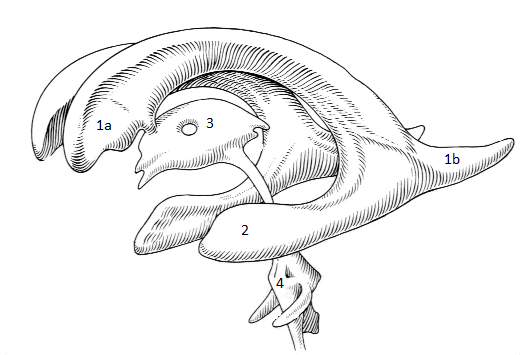
\includegraphics[width=0.75\textwidth]{Logos/Ventrikelsystem_V3.png}
\caption{Zeichnung des Ventrikelsystems  \\  Frei nach \protect\cite{ventrik}} 
\label{fig:ventrik} 
\end{figure}


\subsubsection{Visualisierungen}

Die in diesem Unterkapitel gezeigten Segmentierungen wurde alle auf Volumen mit einer Auflösung von 256x101x256 Pixeln berechnet. In \autoref{fig:norm1_s} und \autoref{fig:norm1_u} ist die Visualisierung eines normalen Ventrikelsystems, in \autoref{fig:norm2_s} und \autoref{fig:norm2_u} die Visualisierung eines weiteren normalen Ventrikelsystems und schließlich in \autoref{fig:atro_s} und \autoref{fig:atro_u} die Visualisierung des Ventrikelsystems eines Patienten mit Atrophie zu sehen. Die Datensätze werden im nächsten Unterkapitel erklärt. Die Abbildungen zeigen Screenshots aus der Darstellung in Unity, jeweils aus den Perspektiven von der Seite und von unten.


\begin{figure}[H]
\begin{minipage}[t]{.5\textwidth}
  \centering
  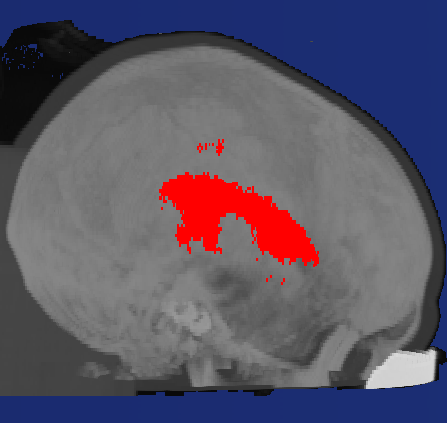
\includegraphics[width=.9\linewidth, height=.9\linewidth]{Logos/Normal1/Seite2.PNG}
  \caption{Visualisierung des \\ ersten normalen \\ Ventrikelsystems von \\ der Seite}
  \label{fig:norm1_s}
\end{minipage}%
\begin{minipage}[t]{.5\textwidth}
  \centering
  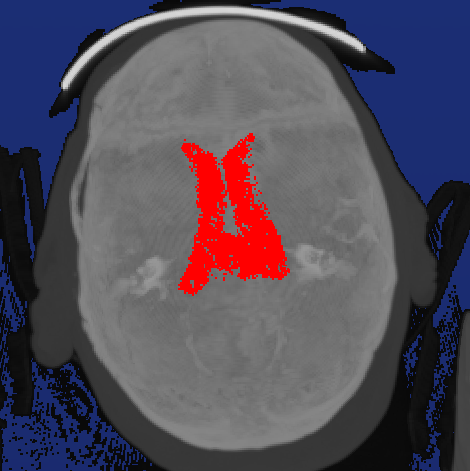
\includegraphics[width=.9\linewidth, height=.9\linewidth]{Logos/Normal1/Unten3.PNG}
  \caption{Visualisierung des \\ ersten normalen \\ Ventrikelsystems von \\ unten}
  \label{fig:norm1_u}
\end{minipage}
\end{figure}

\begin{figure}[H]
\begin{minipage}[t]{.5\textwidth}
  \centering
  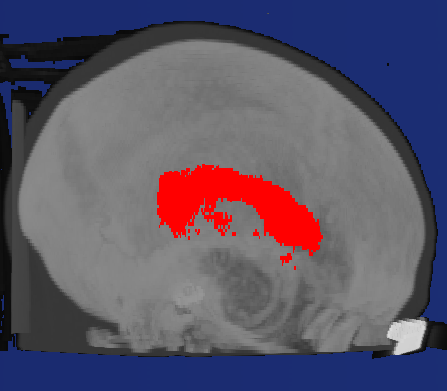
\includegraphics[width=.9\linewidth, height=.9\linewidth]{Logos/Normal2/Seite2.PNG}
  \caption{Visualisierung des \\ zweiten normalen \\ Ventrikelsystems von \\ der Seite}
  \label{fig:norm2_s}
\end{minipage}%
\begin{minipage}[t]{.5\textwidth}
  \centering
  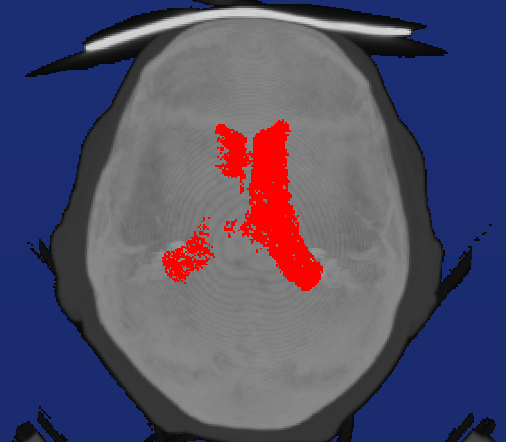
\includegraphics[width=.9\linewidth, height=.9\linewidth]{Logos/Normal2/Unten3.PNG}
  \caption{Visualisierung des \\ zweiten normalen \\ Ventrikelsystems von \\ unten}
  \label{fig:norm2_u}
\end{minipage}
\end{figure}

\begin{figure}[H]
\begin{minipage}[t]{.5\textwidth}
  \centering
  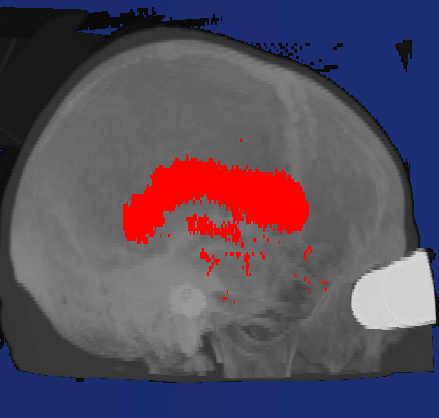
\includegraphics[width=.9\linewidth, height=.9\linewidth]{Logos/Atrophie/Seite2.PNG}
  \caption{Visualisierung des \\ Ventrikelsystems mit \\ Atrophie von der Seite}
  \label{fig:atro_s}
\end{minipage}%
\begin{minipage}[t]{.5\textwidth}
  \centering
  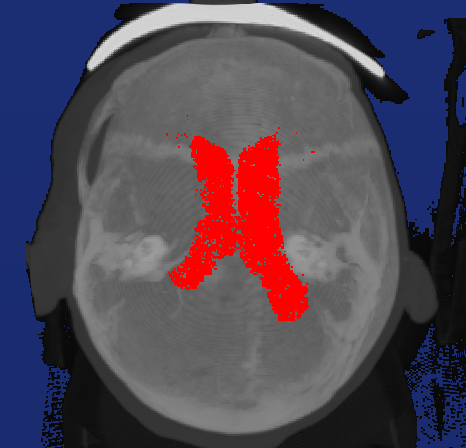
\includegraphics[width=.9\linewidth, height=.9\linewidth]{Logos/Atrophie/Unten3.PNG}
  \caption{Visualisierung des \\ Ventrikelsystems mit \\ Atrophie von unten}
  \label{fig:atro_u}
\end{minipage}
\end{figure}



\subsubsection{Datensätze}

Das Verfahren wurde an 15 verschiedenen CT-Datensätzen der Uni Ulm getestet. Darunter waren verschiedene Ventrikelsysteme. In \autoref{tab:daten} ist eine Auflistung dieser zu sehen.

\begin{table}[H]
\centering
\resizebox{0.65\columnwidth}{!}{
 \begin{tabular}{| c | c | c | c |}
  \hline
  Datensatz (ID) & Anzahl \\ \hline
   Normale Ventrikel (D1) & 3  \\ \hline
   Schlanke Ventrikel (D2) & 4  \\ \hline
   Mittellinienshift (D3) & 2  \\ \hline
   Deformiertes (D4) & 1 \\ \hline
   Atrophie (D5) & 2  \\ \hline
   Hydrocephalus-Ventrikelblut (D6) & 1 \\ \hline
   Subarachnoidale Einblutung (D7) & 1 \\ \hline
   Blut-resorbiert (D8) & 1  \\ \hline
 \end{tabular}
 }
\caption{Verwendeten Datensätze}
\label{tab:daten}
\end{table}



Da die Aufgabe das Ventrikelsystem anhand von CT-Daten automatisiert zu segmentieren sehr komplex ist, kam es bei Patienten veränderten Ventrikelsystemen, z.B.  durch Verformung oder Krankheit, zu Problemen.
Das Verfahren erkennt Strukturen anhand ihrer Grenzen. Deshalb war es nicht möglich, bei ''D2: Schlanke Ventrikel'' zu einer erfolgreichen Segmentierung zu gelangen. Sehr dünne Strukturen anhand von CT-Daten zu erkennen, ist kaum bis gar nicht realisierbar, da diese nicht hochauflösend genug sind. Dieses Problem tritt ebenfalls bei ''D3: Mittellinienshift'' und  ''D4: Deformiert'' auf. Ein Mittellinenshift bezeichnet die Verschiebung der Mittellinie und eine Verformung des Ventrikelsystems, was beispielsweise durch Gewalteinwirkung auf den Kopf hervorgerufen werden kann. Bei ''D4: Deformiert'' wird das System aufgrund eines Tumors im Gehirn stark verformt. Durch diese Verformungen ist das Ventrikelsystem allgemein sehr schlecht bis gar nicht von umliegenden Strukturen abgrenzbar.
\newline
Atrophie ist ein oft durch das Alter verursachter Schwund an Gehirnmasse. Bei diesem weiten sich alle Ventrikel und es ist im Allgemeinem mehr Liquor im Gehirn zu finden. Dadurch war es bei einem der beiden Datensätze von D5 nicht möglich, eine Segmentierung vorzunehmen, da durch die viele Flüssigkeit im Gehirn die Grenze zwischen dem System und der umliegenden Hirnmasse stark verschwammen.
Ein ähnliches Problem entstand bei ''D6: Hydrocephalus-Ventrikelblut'' und ''D7: Subarachnoidale Einblutung'', bei denen die Ventrikel fast vollständig mit Blut vollgelaufen sind. Dadurch war es nicht möglich das System vom restlichen Gehirn abzugrenzen.
Beim ''D8: Blut-resorbiert'' handelt es sich um den D6 Datensatz, nachdem das Blut entfernt wurde. Das Ventrikelsystem hat sich jedoch noch nicht wieder vollständig mit Liquor gefüllt, was erneut keine Segmentierung zuließ.
Der dritte D1 Datensatz hat eine Verkalkung des liquorproduzierenden Plexus, weshalb auch hier weniger Liquor in den Ventrikeln zu finden war.



\subsubsection{Auswertung}

Um die Qualität der erzeugten Segmentierungen zu evaluieren, wurde ein Arzt von der Uniklinik Ulm interviewt. Diesem wurden die drei gezeigten Visualisierungen direkt in Unity vorgeführt. Während der Vorführung konnte der Mediziner selbst die Kamera durch die Darstellung lenken und das Ergebnis aus verschiedenen Blickwinkeln betrachten.
\newline
Anschließend bewertete er die Qualität der Ergebnisse, indem er drei verschiedenen Fragen zu den Darstellungen beantwortete. Er musste dabei seine Antwort immer auf einer Skala von 1 bis 5 angeben.
Die Fragen lauteten:
\begin{itemize}
	\item 1) Wie gut ist das Ventrikelsystem bei der Visualisierung zu erkennen? \newline sehr schlecht(1), sehr gut(5)
	\item 2) Wird das Ventrikelsystem in der Visualisierung vollständig dargestellt? \newline überhaupt nicht vollständig(1), vollständig(5)
	\item 3) Wie genau ist das Ventrikelsystem segmentiert? \newline überhaupt nicht segmentiert(1), ausschließlich das Ventrikelsystem ist segmentiert(5)
\end{itemize}


Die Antworten des Arztes werden in \autoref{tab:ergebnis_arzt} gezeigt. Allgemein merkte der Mediziner an, dass bei jeder Visualisierung, die durch das Verfahren erzeugt wurde, nur der linke und rechte Seitenventrikel zu sehen war. Die deutlich schmaleren dritten und vierten Ventrikel und die Unterhörner der Seitenventrikel fehlten bei den Darstellungen. Er erklärte jedoch, dass diese bei einem gesunden Menschen sehr dünn und deshalb anhand von CT-Daten schwer bis gar nicht zu segmentieren seien. Weiterhin sind, wie schon erwähnt, die Seitenventrikel entscheidend für eine erfolgreiche Punktion.
\newline
Deshalb bezog sich die Beantwortung der zweiten Frage nach der Vollständigkeit des Ventrikelsystems lediglich auf die Vollständigkeit der beiden Seitenventrikel.

\begin{table}[h]
\centering
\tiny
\resizebox{\columnwidth}{!}{
 \begin{tabular}{| c | c | c | c |}
  \hline
  Ventrikelsystem & 1. Frage & 2.Frage & 3. Frage\\ \hline
  Normal 1 & 4 & 4 & 3 \\ \hline
  Normal 2 & 4 & 2 & 3\\ \hline
  Atrophie & 4 & 3 & 2 \\ \hline
 \end{tabular}
 }
\caption{Ergebnisse des Interviews mit einem Arzt}
\label{tab:ergebnis_arzt}
\end{table}


Die Bewertung des ersten normalen Ventrikelsystems fiel positiv aus mit 11 von 15 möglichen Punkten. Das Ventrikelsystem war klar und deutlich zu erkennen, jedoch fehlte ein Teil der Hinterhörner. Bis auf diese waren die Seitenventrikel vollständig zu sehen. Allerdings war die Segmentierung nicht exakt, da es mehrere kleine Ausreißer gab.
\newline
Das zweite normale Ventrikelsystem war ebenfalls klar zu erkennen. Jedoch wurde fast ausschließlich der linke Seitenventrikel segmentiert. Die Bewertung der Vollständigkeit fiel mit einer vier hoch aus, da der eine Seitenventrikel sehr klar, deutlich und umfassend zu sehen war.Dieser war besser und glatter als die des ersten normalen Ventrikelsystems sein, da auch das Hinterhorn zu erkennen ist. 
\newline
In einem Gehirn eines unter Atrophie leidenden Menschen ist deutlich mehr Liquor als bei einem gesunden Menschen zu finden. Diese Flüssigkeiten werden vom Verfahren ebenfalls erkannt, weshalb die Segmentierung etwas verschwommen erscheint und nicht die kompletten Seitenventrikel erfasst werden. Jedoch vermutete der Arzt, dass viele der Ausreißer zum dritten Ventrikel gehören könnten, da sich dieses, wie alle Ventrikel bei einer Atrophie, weitet. Trotz der Flüssigkeiten im Gehirn war das Ventrikelsystem in der Darstellung deutlich auszumachen.
\newline
Im Allgemeinen waren die Darstellungen nicht glatt genug und es existieren viele Ausreißer. Das Ventrikelsystem war jedoch bei allen Visualisierungen eindeutig zu erkennen und die Aufgabe das System zu segmentieren war gelungen.


\begin{figure}[h]
\begin{minipage}[t]{.5\textwidth}
  \centering
  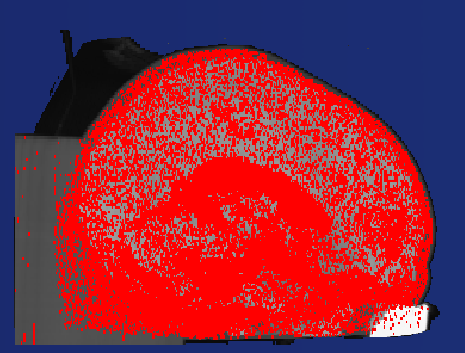
\includegraphics[width=.9\linewidth, height=.9\linewidth]{Logos/Normal1_Unity/Seite.PNG}
  \caption{Visualisierung des \\ ersten normalen \\ Ventrikelsystems von \\ der Seite mithilfe \\ von Unity}
  \label{fig:unity_s}
\end{minipage}%
\begin{minipage}[t]{.5\textwidth}
  \centering
  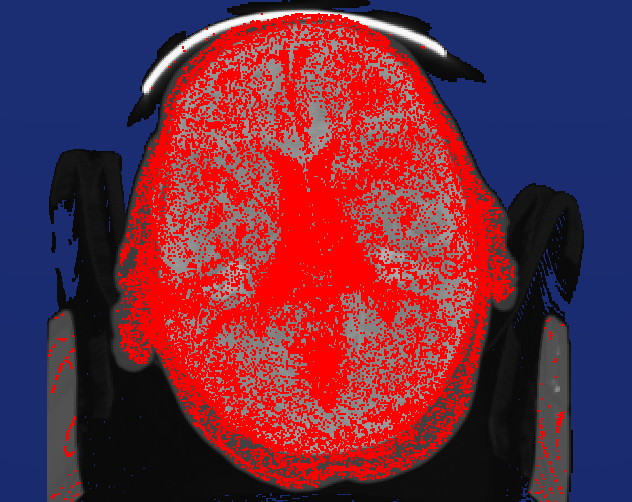
\includegraphics[width=.9\linewidth, height=.9\linewidth]{Logos/Normal1_Unity/Unten3.PNG}
  \caption{Visualisierung des \\ ersten normalen \\ Ventrikelsystems von \\ unten mithilfe \\ von Unity}
  \label{fig:unity_u}
\end{minipage}
\end{figure}


Zur weiteren Auswertung der Ergebnisse wurde das erste normale Ventrikelsystem aus \autoref{fig:norm1_s} und \autoref{fig:norm1_u} in Unity und mit der MITK-Workbench, die auch zum Umwandeln der DICOM-Dateien benutzt wurde, visualisiert.
\newline
In Unity wurde dabei die Erweiterung zum Hervorheben von Wertebereichen benutzt. Diese wurde auf 1025 bis 1030 eingestellt, da das Ventrikelsystem Intensitätswerte in diesem Bereich hat. Dieses Vorgehen entspricht einer simplen eindimensionalen Transferfunktion, die abhängig von den Intensitätswerten Voxel, einfärbt.
Die Ergebnisse sind in \autoref{fig:unity_s} und \autoref{fig:unity_u} zu sehen. Das Ventrikelsystem ist zwar zu sehen, es gibt jedoch sehr viele Ausreißer, die es fast unmöglich machen, die Ventrikel eindeutig zu erkennen. Diese simple Vorgehensweise erzielt kein gewünschtes Ergebnis.


\begin{figure}[h]
\begin{minipage}[t]{.5\textwidth}
  \centering
  
\includegraphics[width=.9\linewidth, height=.9\linewidth]{Logos/Normal1_MITK/Oben.PNG}
  \caption{Visualisierung des \\ ersten normalen \\ Ventrikelsystems von \\ oben mithilfe \\ von MITK}
  \label{fig:mitk_o}
\end{minipage}%
\begin{minipage}[t]{.5\textwidth}
  \centering
  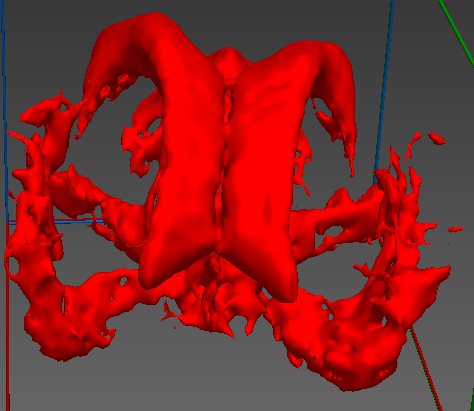
\includegraphics[width=.9\linewidth, height=.9\linewidth]{Logos/Normal1_MITK/Schraeg_Vorne.PNG}
  \caption{Visualisierung des \\ ersten normalen \\ Ventrikelsystems von \\ vorne mithilfe \\ von MITK}
  \label{fig:mitk_v}
\end{minipage}
\end{figure}


In der MITK-Workbench gibt es verschiedene Segmentierungstools. Darunter ist ein Region Growing Tool, bei dem der Nutzer einen \textit{seed} Punkt in den Schnittbildern wählen kann. Über die verwendete Kostenfunktion gibt es keine Informationen.
Anschließend können die Löcher der Auswahl mit einem \textit{closing} Filter geschlossen und mit einem weiteren Tool ein geglättete 3D Ansicht des Ergebnis erzeugt werden. Eine genaue Beschreibung über das Anwenden der Tools ist im Anhang dieser Arbeit zu finden.
\newline
Screenshots der Ergebnisse sind in \autoref{fig:mitk_o} und \autoref{fig:mitk_v} zu sehen. In dem von der Workbench erzeugte Ergebnis ist das Ventrikelsystem gut zu erkennen. Die Seitenventrikel sind vollständig und besitzen eine glatte Oberfläche. Sogar große Teile des dritten und vierten Ventrikels sind Teil der Segmentierung.
Allerdings sind auch ganze Bereiche hervorgehoben, die nicht zum Ventrikelsystem gehören. Diese könnten vom Benutzer manuell in jedem Schichtbild des Datensatzes entfernt werden, was jedoch sehr zeitaufwändig wäre.


\subsection{Nutzerstudie}


Im Rahmen der Evaluation der Benutzerfreundlichkeit des Verfahrens wurde eine kleine Nutzerstudie mit 5 Teilnehmern durchgeführt. Die Probanden waren alle Studenten aus verschiedenen Studiengängen im Alter zwischen 22 und 26 Jahren.
Als erstes wurde den Teilnehmern der Ablauf und die vom Benutzer erforderlichen Schritte, um eine Visualisierung des Ventrikelsystems zu erhalten, mittels einer Vorführung durch den Interviewer gezeigt.
Anschließend sollten die Probanden selbst das eben gelernte anwenden und das Programm selber ausführen. Dabei bekamen sie, wenn sie nicht weiterwussten, Hilfe vom Versuchsleiter.
\newline
Hinterher füllten die Teilnehmer einen NASA-TLX Bogen zu der Aufgabe aus. Dieser besteht aus zwei Parts. Als erstes muss der Befragte in den Kategorien Geistige Anforderung, Körperliche Anforderung, Zeitliche Anforderung, Leistung, Anstrengung und Frustration die auszuführende Aufgabe jeweils auf einer Skala von 5 bis 100 bewerten. Die Werte der Skalen wachsen dabei in Fünfer Schritten an. Diese Bewertung ergibt hinterher die Gewichtung der Kategorien.
Als zweites werden alle Kategorien paarweise miteinander verglichen und der Probanden muss angeben, welcher der beiden Kategorien für das Lösen der Aufgabe bedeutsamer war. Dadurch erhält jede Kategorie eine Anzahl an Klicks.
Anschließend wird die Klickzahl durch 15, die Anzahl aller Klicks geteilt. Dies ergibt die die Wichtung der Kategorie. Diese Wichtungen werden mit deren jeweiligen Gewichtungen multipliziert und die Ergebnisse zur Gesamtbeanspruchung der Aufgabe aufaddiert.
Die durchschnittlichen Ergebnisse der einzelnen Kategorien werden in \autoref{tab:ergebnis_nasa} gezeigt.


\begin{table}[H]
\centering
\resizebox{\columnwidth}{!}{
 \begin{tabular}{| c | c | c | c |}
  \hline
  Kategorie & Gewichtung & Klicks & Wichtung \\ \hline
  Geistige Anforderung & 39 & 4,8 & 0,32 \\ \hline
  Körperliche Anforderung & 23 & 1,8 & 0,12\\ \hline
  Zeitliche Anforderung & 29 & 1,2 & 0,078 \\ \hline
  Leistung & 25 & 2,4 & 0,156\\ \hline
  Anstrengung & 36 & 2,4 & 0,156\\ \hline
  Frustration & 35 & 2,4 & 0,156\\ \hline 
 \end{tabular}
 }
\caption{Durchschnittlichen Ergebnisse des NASA-TLX Bogens}
\label{tab:ergebnis_nasa}
\end{table}


Der durchschnittliche Wert für die Gesamtbeanspruchung lag bei 38,32. 


Zunächst werden die Ergebnisse des ersten Teils betrachtet. Hierbei fällt als erstes auf, dass die bei Kategorien Geistige Anforderung, Anstrengung und Frustration durchschnittlichen die höchsten Bewertungen abgegeben wurden.
Bei der Geistigen Anforderung und der Frustration gaben vor allem die Teilnehmer ohne oder mit nur wenig Programmiererfahrung höhere Werte an. Bei der Kategorie Anstrengung ist anzumerken, dass von zwei Probanden deutlich höhere Werte als vom Rest gegeben wurde.
Alle anderen Kategorien wurden in etwa ähnlich bewertet.
\newline
Als nächstes werden die Ergebnisse des zweiten Parts diskutiert. Die höchste durchschnittliche Klickzahl wurde von der Kategorie Geistige Anforderung erzielt. Unabhängig von den Programmierkenntnissen der Probanden wurde diese Kategorie als die deutlich bedeutsamste angesehen.
Die anderen Kategorien unterscheiden sich nur geringfügig und hatten meist Klickzahlen zwischen null und drei.
\newline
Als letztes wird die Gesamtbeanspruchung betrachtet. Dieser unterscheidet sich bei den Teilnehmern vor allem durch die unterschiedliche Bewertung der Kategorien Geistige Anforderung und Frustration sehr stark von einander.
Die berechneten Gesamtbeanspruchungen lagen bei 14,6\; 27,3\; 40\; 40,6 und 63. Dies zeigt den großen Unterschied zwischen den Personen, die viel Programmiererfahrungen besitzen, und denen, die wenig oder noch nie programmiert haben.
Die Benutzung einer Konsole fiel den Unerfahrenen vergleichsweise sehr schwer. Des Weiteren ist die Notwendigkeit die richtigen Suffixe und das $u$ beim \textit{ClusterVolume} Modul angeben zu müssen eine Hürde. Weiterhin wäre es einfacher, wenn nur ein Programm verwendet werden müsste.
\newline 
Trotz der Schwierigkeiten gaben alle Probanden an, auch jene ohne Programmiererfahrung, dass sie die Aufgabe mit einer gut erklärten, ausführlichen Dokumentation alleine, ohne weitere Hilfe durchführen könnten.

\subsection{Berechnungszeit}

Die in diesem Unterkapitel vorgestellten Zeitmessungen wurden alle auf einem Computer mit einem 3.70GHz  Intel Core(TM) i7-8700K CPU mit 32GB RAM ausgeführt.
Um die Berechnungszeit des Systems evaluieren zu können, wurde die Kalkulation des gesamten Clusteringverfahrens sowie die Berechnung des LH-Histogramms auf drei Volumen verschiedener Größen durchgeführt. Damit der Vergleich nicht von unterschiedlichen Volumendaten verfälscht wird, wurden alle Volumen aus dem gleichen CT-Datensatz generiert.
\newline
Dabei wurde die Originalgröße, die ein Auflösung von 512x201x512 Voxeln besitzt, mithilfe des Resamplemoduls des Helpers verkleinert. Die beiden anderen Volumengrößen haben dabei die  Hälfte, mit 256x101x256 Voxeln, und Dreiviertel, mit 384x151x384 Voxeln, der Auflösungen des Originalvolumens.
Es war geplant, dass noch ein viertes Volumen zum Vergleich hinzugezogen wird. Jedoch war es aus einem unbekannten Grund nicht möglich, die beiden Berechnungen mit dem gevierteltem Volumen durchzuführen.
Des Weiteren funktionierte beim Originalvolumen lediglich die Berechnung des LH-Histogramms. Die Kalkulation des Clusteringverfahrens war nicht möglich, vermutlich weil es bei dieser hohen Auflösung zu viele Daten für die aktuelle Implementierung zu berechnen gab.
Die Berechnungszeit hängt stark von der Größe des Eingabevolumens ab. Dies ist in \autoref{tab:ueberblick_zeit} sehr gut zu erkennen. Sie gibt einen Überblick über die  Berechnungszeiten der verschiedenen Volumengrößen.


\begin{table}[h]
\centering
\resizebox{\columnwidth}{!}{
 \begin{tabular}{| c | c | c | c |}
  \hline
  Volumengröße & LH-Histogramm $[s]$ & Komplettes Verfahren $[s]$ \\ \hline
  Halbes Volumen (256x101x256)  & 30 &  50	\\ \hline
  Dreiviertel Volumen (384x151x384)  & 90 &  380	\\ \hline
  Ganzes Volumen (512x201x512) & 225 & -	\\ \hline
 \end{tabular}
 }
\caption{Überblick über die Berechnungszeiten der verschiedenen Volumengrößen}
\label{tab:ueberblick_zeit}
\end{table}


Dabei ist wichtig zu beachten, dass die Zeit zur Berechnung der LH-Histogramme die gleiche Zeit wie die Kalkulation der LH-Werte im gesamten Verfahren benötigt. Die Berechnungsdauer der Gradienten ist hierbei zirka doppelt so lange wie die der LH-Werte. Wird die Berechnungszeit des Histogramms von der Kalkulationszeit des gesamten Verfahrens abgezogen, ergibt dies die Zeit, die die beiden Clusteringschritte benötigen.

\begin{table}[h]
\centering
\resizebox{\columnwidth}{!}{
 \begin{tabular}{| c | c | c | c |}
  \hline
  Volumengröße & LH-Histogramm $[Voxel/s]$ & Clustering $[Voxel/s]$ \\ \hline
  256x101x256  & $220 * 10^3$ &  $330 * 10^3$ \\ \hline
  384x151x384  & $247 * 10^3$ &  $76 * 10^3$	\\ \hline
  512x201x512 & $234 * 10^3$ & -	\\ \hline
 \end{tabular}
 }
\caption{Überblick über die Berechnungsraten der verschiedenen Volumengrößen}
\label{tab:ueberblick_rate}
\end{table}



Eine interessante Beobachtung hierbei war, dass die Berechnung der LH-Histogramme abhängig von der Anzahl der Voxel in etwa gleich schnell abläuft. Das halbe Volumen hat eine Gesamtvoxelzahl von ungefähr 6,6 Millionen, das 75\% Volumen von zirka 22,2 Millionen und das Original von ca. 52,6 Millionen Voxeln.
Die Anzahl der bearbeiteten Voxel pro Sekunde bei der Berechnung des LH-Histogramms sowie der Clusteringschritte ist in \autoref{tab:ueberblick_rate} zu sehen.
\newline
Dabei ist zu beobachten, dass beim der Kalkulation der LH-Histogramme keine großen Unterschiede zwischen den Raten existiert.
Beim halben Volumen werden etwa 220 Tausend, beim dreiviertel Volumen ungefähr 247 Tausend und beim original Volumen 234 Tausend Voxel pro Sekunde bearbeitet. Der kleine Unterschied in der Rate lässt sich einerseits durch von der Volumengröße unabhängige Berechnungen und andererseits durch Messfehler erklären. Folglich kann die Aussage getroffen werden, dass die Berechnungszeit der LH-Werte bei dieser Implementierung in etwa linear mit der Anzahl an Eingabepixeln wächst.
\newline
Auf der anderen Seite ist jedoch auch zu erkennen, dass die beiden Clusteringschritte mit zunehmender Eingabegröße deutlich langsamer werden. Das Clustering des halben Volumens dauerte 20 Sekunden und hat damit eine Verarbeitungsrate von zirka 330 Tausend Pixeln pro Sekunde. Hingegen dauert es beim dreiviertel Volumen 290 Sekunden und erreicht damit gerade einmal eine Rate von 76 Tausend Pixeln pro Sekunde. Es benötigt also 14,5 mal so viel Zeit für die 3,3 fache Anzahl an Pixeln.














































